\documentclass[12pt, titlepage]{article}

\usepackage{fullpage}
\usepackage[round]{natbib}
\usepackage{multirow}
\usepackage{booktabs}
\usepackage{tabularx}
\usepackage{graphicx}
\usepackage{float}
\usepackage{hyperref}
\hypersetup{
    colorlinks,
    citecolor=blue,
    filecolor=black,
    linkcolor=red,
    urlcolor=blue
}

%% Comments

\usepackage{color}

\newif\ifcomments\commentstrue %displays comments
%\newif\ifcomments\commentsfalse %so that comments do not display

\ifcomments
\newcommand{\authornote}[3]{\textcolor{#1}{[#3 ---#2]}}
\newcommand{\todo}[1]{\textcolor{red}{[TODO: #1]}}
\else
\newcommand{\authornote}[3]{}
\newcommand{\todo}[1]{}
\fi

\newcommand{\wss}[1]{\authornote{blue}{SS}{#1}} 
\newcommand{\plt}[1]{\authornote{magenta}{TPLT}{#1}} %For explanation of the template
\newcommand{\an}[1]{\authornote{cyan}{Author}{#1}}

%% Common Parts

\newcommand{\progname}{ProgName} % PUT YOUR PROGRAM NAME HERE
\newcommand{\authname}{Team \#, Team Name
\\ Student 1 name
\\ Student 2 name
\\ Student 3 name
\\ Student 4 name} % AUTHOR NAMES                  

\usepackage{hyperref}
    \hypersetup{colorlinks=true, linkcolor=blue, citecolor=blue, filecolor=blue,
                urlcolor=blue, unicode=false}
    \urlstyle{same}
                                


\newcounter{acnum}
\newcommand{\actheacnum}{AC\theacnum}
\newcommand{\acref}[1]{AC\ref{#1}}

\newcounter{ucnum}
\newcommand{\uctheucnum}{UC\theucnum}
\newcommand{\uref}[1]{UC\ref{#1}}

\newcounter{mnum}
\newcommand{\mthemnum}{M\themnum}
\newcommand{\mref}[1]{M\ref{#1}}

\begin{document}

\title{System Design for \progname{}} 
\author{\authname}
\date{\today}

\maketitle

\pagenumbering{roman}

\section{Revision History}

\begin{tabularx}{\textwidth}{p{3cm}p{2cm}X}
\toprule {\bf Date} & {\bf Version} & {\bf Notes}\\
\midrule
Date 1 & 1.0 & Notes\\
Date 2 & 1.1 & Notes\\
\bottomrule
\end{tabularx}

\newpage

\section{Reference Material}

This section records information for easy reference.

\subsection{Abbreviations and Acronyms}

\renewcommand{\arraystretch}{1.2}
\begin{tabular}{l l} 
  \toprule		
  \textbf{symbol} & \textbf{description}\\
  \midrule 
  \progname & The Software Engineering Capstone Project Course at McMaster University\\
  Figma & A collaborative web application for interface design\\
  \bottomrule
\end{tabular}\\

\newpage

\tableofcontents

\newpage

\listoftables

\listoffigures

\newpage

\pagenumbering{arabic}

\section{Introduction}
This document describes the design for the CodeChamp system. The design document is split up into three documents, the \href{https://github.com/Tamas-Leung/CodeChamp/tree/main/docs/Design/MIS}{Module Interface Specification}, \href{https://github.com/Tamas-Leung/CodeChamp/tree/main/docs/Design/MG}{Module Guide} and the system design document. Other relevant documentation is listed below:
\begin{enumerate}
    \item \href{https://github.com/Tamas-Leung/CodeChamp/tree/main/docs/DevelopmentPlan}{Development Plan}
    \item \href{https://github.com/Tamas-Leung/CodeChamp/tree/main/docs/SRS}{System Requirements Specification} 
    \item \href{https://github.com/Tamas-Leung/CodeChamp/blob/main/docs/HazardAnalysis/HazardAnalysis.md}{Hazard Analysis} 
    
\end{enumerate}

\section{Purpose}

This document is written to describe the architecture and the design decisions in the CodeChamp system. Primarily, it introduces the scope of the system to demonstrate the possible interactions with the outside world. Moreover, it gives an overview of the project, recounting the important components from a high level and describing the normal behavior of the system. Additionally, it gives a high-level overview of the event handling mechanisms in place for undesired behavior. Since the CodeChamp system is user-centric, the document also describes mock-ups for the user interface design of the system. Finally, a timeline is given for the implementation of the system. 


\section{Scope}


\begin{figure}[H]
\centering
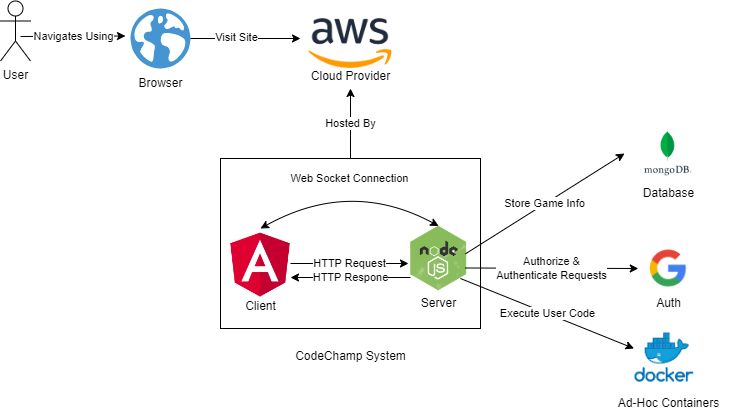
\includegraphics[scale=0.65]{Design/SystDesign/SystemBoundary.png}
\caption{Context Diagram for the CodeChamp System}
\end{figure}

\section{Project Overview}

\subsection{Normal Behaviour}

\begin{enumerate}
    \item User navigates to site using web browser
    \item User logs into the application
    \item User creates/joins a game
    \item The game starts once the lobby is ready
    \item User plays the game by attempting to solve the problem
    \item User proceeds to the next round upon successfully completing a round
    \item User loses after being unable to complete a round/User wins by winning all the rounds
    \item User checks his personal statistics and match history by going to the Home Page and click on the personal profile button
    \item User checks the leaderboard by going to the Home Page and click on the leaderboard button
\end{enumerate}

\subsection{Undesired Event Handling}
Undesired events will be passed onto the front-end to be handled. The front-end will display a dialog mentioning the event in natural language and log the event in details.

\subsection{Component Diagram}

\begin{figure}[H]
\centering
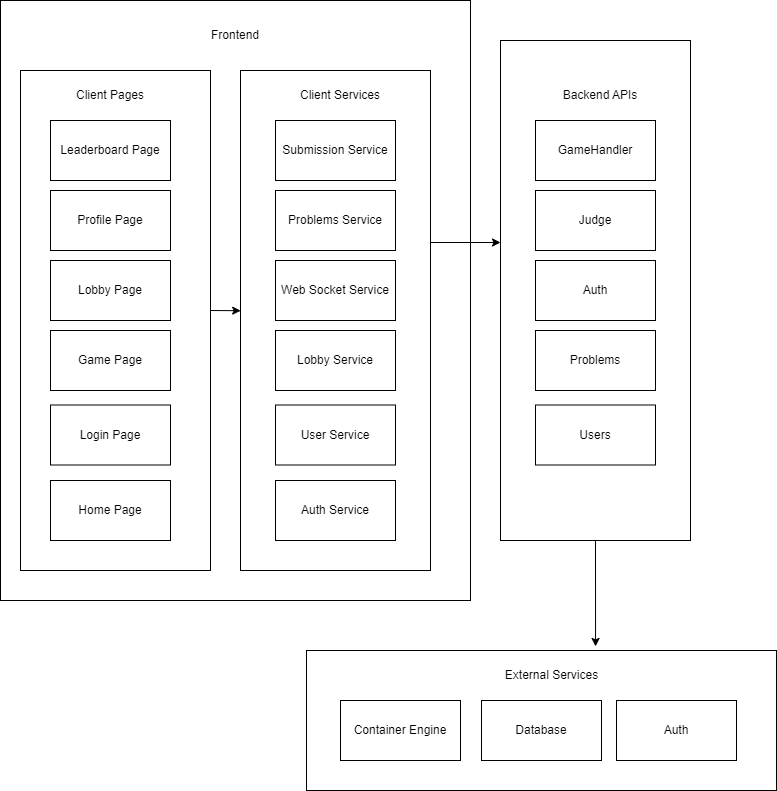
\includegraphics[width=0.8\textwidth]{Design/SystDesign/ComponentDiagram.png}
\caption{Component Diagram for the CodeChamp System}
\end{figure}

\subsection{Connection Between Requirements and Design} \label{SecConnection}

\begin{table}[H]
\centering 
\begin{tabular}{p{0.2\textwidth} p{0.6\textwidth}}
\toprule
\textbf{Req.} & \textbf{Decisions}\\
\midrule
NFR11 & Users use username, password, email to create accounts, Google Oauth is used as implementation\\ 
FR6, FR14, FR15 & Using containerized engine to run code compilation, avoiding effects of compiling malicious code\\
FR3 & Game cuts player count in half in each round to have at most 4 rounds\\
FR.23 & Using unique yet human readable IDs/lobby codes for ease of joining. \\
FR.13 & The system allows developers to create/modify tests through network calls \\
FR.1 & System uses random matchmaking instead of the other option, skill based match making. \\
\hline
\end{tabular}
\caption{Requirements and Design Decisions made}
\label{TblRT2}
\end{table}

% \wss{The intention of this section is to document decisions that are made
%   ``between'' the requirements and the design.  To satisfy some requirements,
%   design decisions need to be made.  Rather than make these decisions implicit,
%   they are explicitly recorded here.  For instance, if a program has security
%   requirements, a specific design decision may be made to satisfy those
%   requirements with a password.}

\section{User Interfaces}

The following mock-ups were produced using Figma for the CodeChamp user interface: 

\begin{figure}[H]
\centering
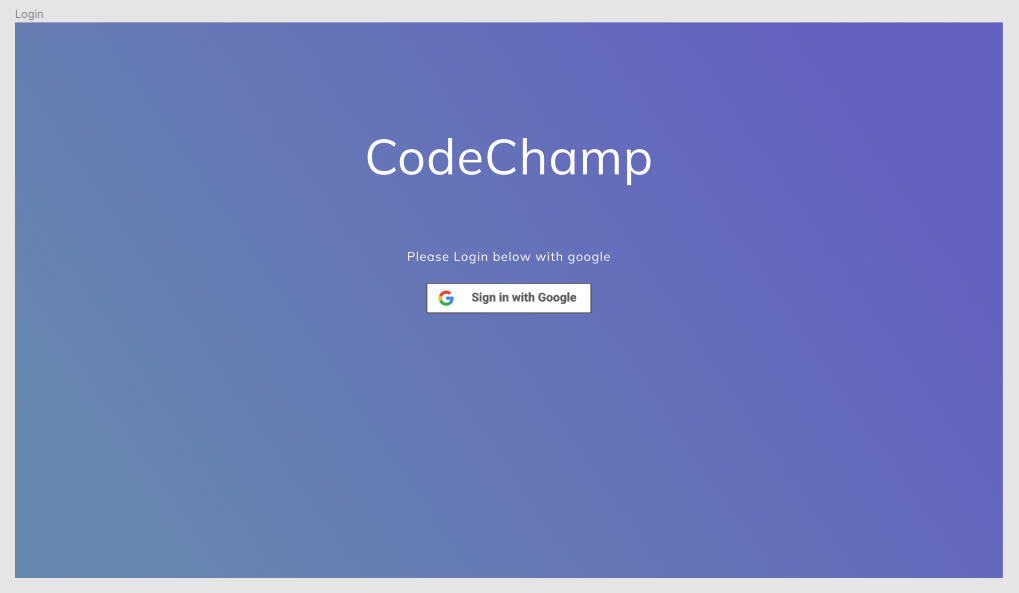
\includegraphics[width=0.8\textwidth]{Design/SystDesign/LoginPage.png}
\caption{Mock-up for CodeChamp's Login Page}
\end{figure}

\begin{figure}[H]
\centering
\includegraphics[width=0.8\textwidth]{Design/SystDesign/HomePage.png}
\caption{Mock-up for CodeChamp's Home Page}
\end{figure}

\begin{figure}[H]
\centering
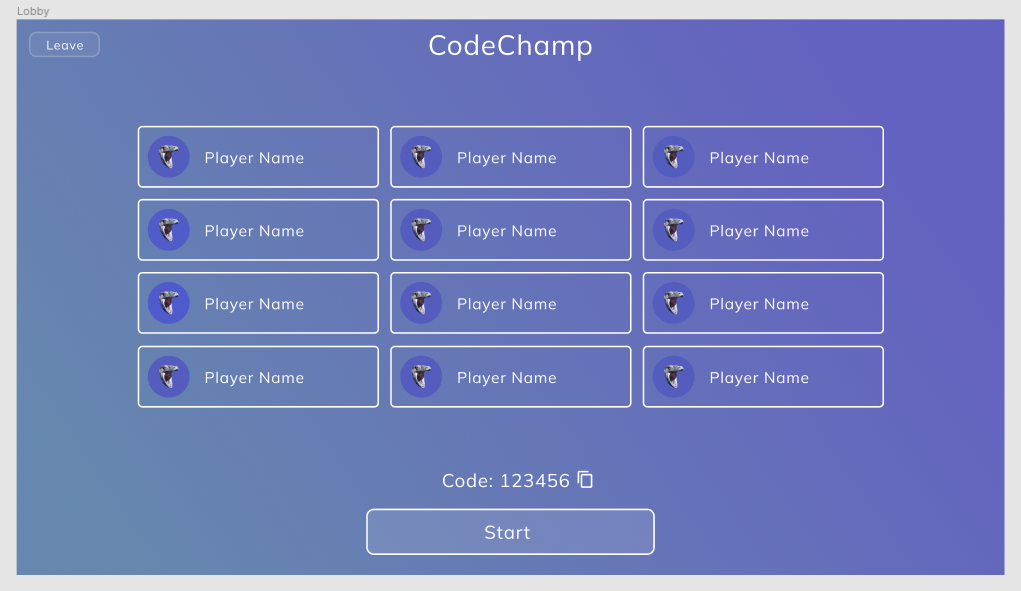
\includegraphics[width=0.8\textwidth]{Design/SystDesign/LobbyPage.png}
\caption{Mock-up for CodeChamp's Lobby Page}
\end{figure}

\begin{figure}[H]
\centering
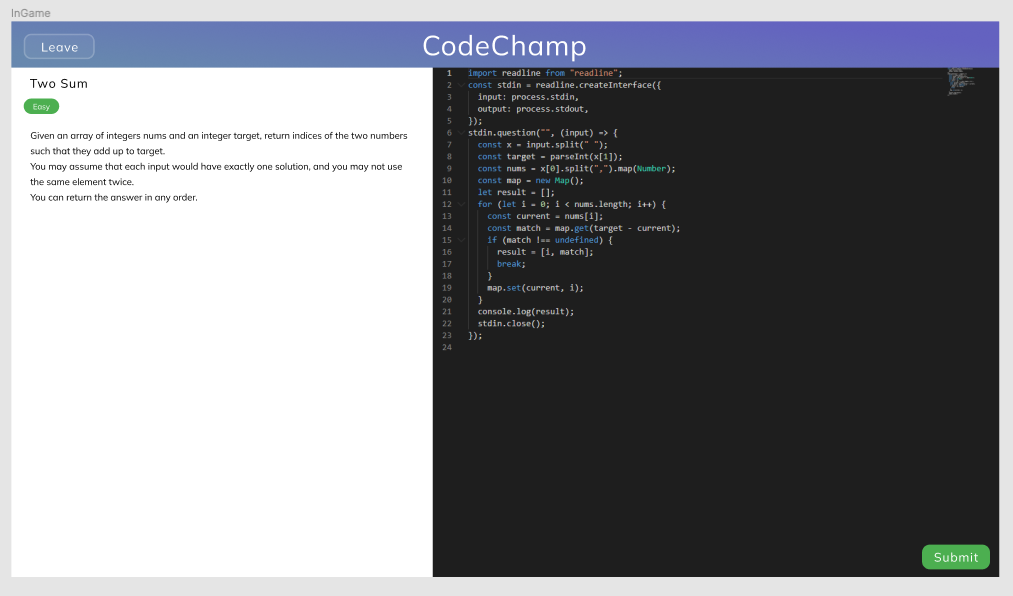
\includegraphics[width=0.8\textwidth]{Design/SystDesign/GamePage.png}
\caption{Mock-up for CodeChamp's Game Page}
\end{figure}

\begin{figure}[H]
\centering
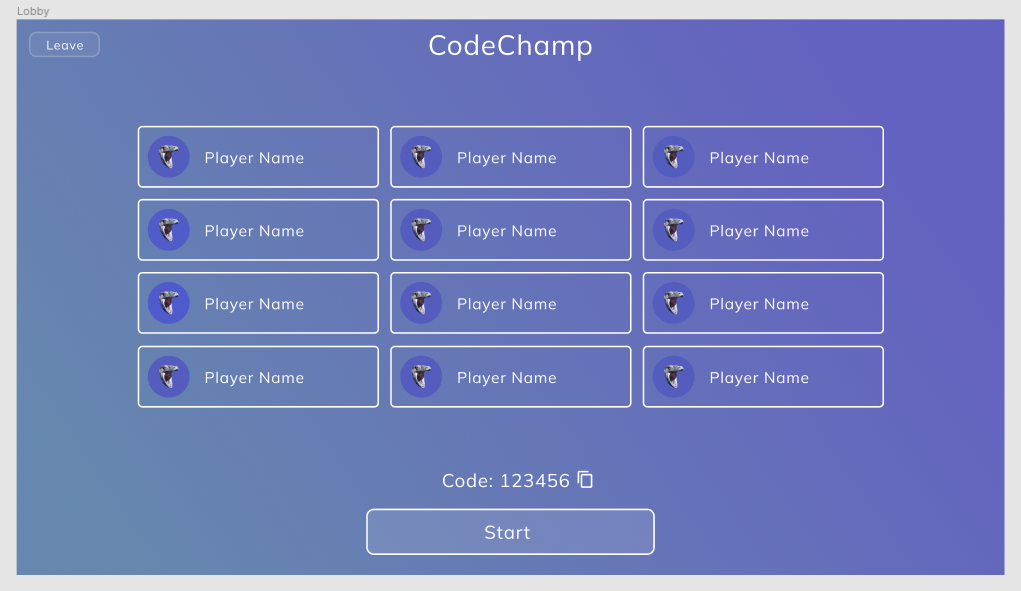
\includegraphics[width=0.8\textwidth]{Design/SystDesign/LeaderboardPage.png}
\caption{Mock-up for CodeChamp's Leaderboard Page}
\end{figure}

\begin{figure}[H]
\centering
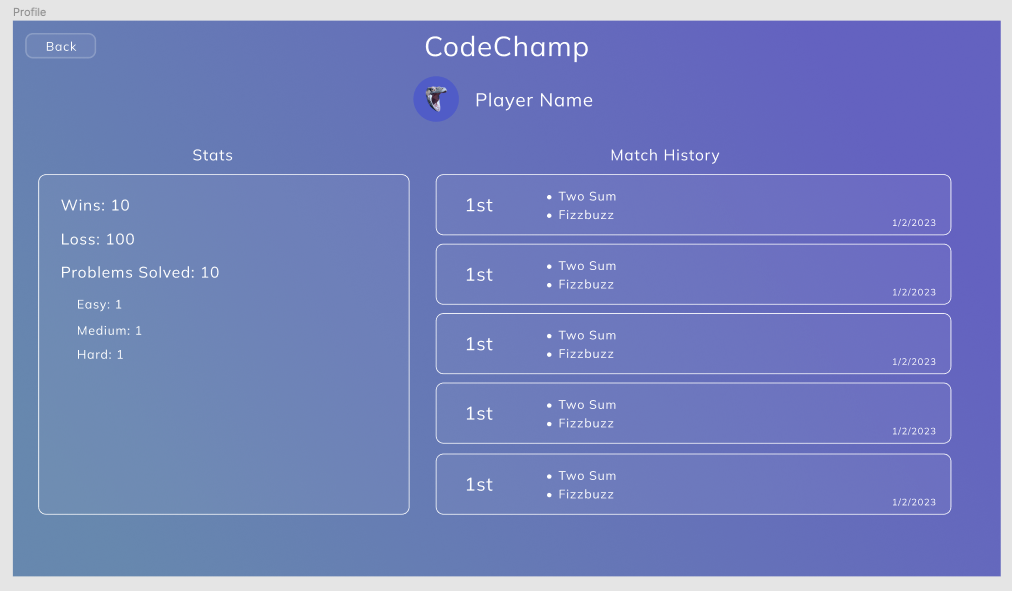
\includegraphics[width=0.8\textwidth]{Design/SystDesign/ProfilePage.png}
\caption{Mock-up for CodeChamp's Profile Page}
\end{figure}

\begin{figure}[H]
\centering
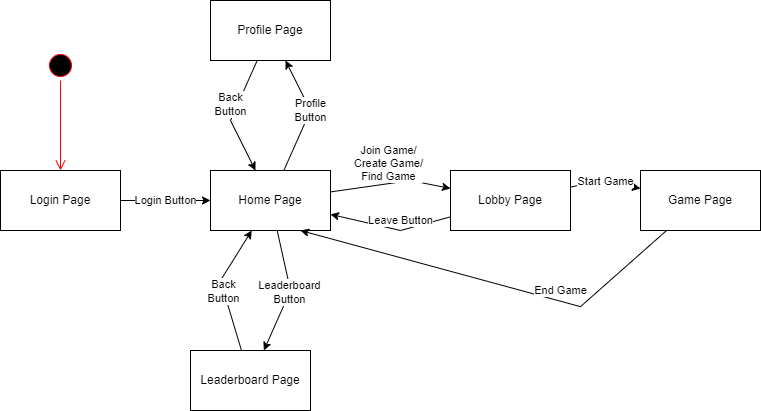
\includegraphics[width=1\textwidth]{Design/SystDesign/State.png}
\caption{State Machine for front end pages}
\end{figure}

\section{Design of Hardware}

N/A

\section{Design of Electrical Components}

N/A

\section{Design of Communication Protocols}

Using HTTPS to send requests and retrieve data from the servers and database. For bi-directional messaging between clients and servers, WebSocket technology is used. Technologies are not implemented by the CodeChamp team.

\section{Timeline}


\begin{table}[H]
\centering
\begin{tabular}{p{0.35\textwidth} p{0.3\textwidth}  p{0.3\textwidth}}
\toprule
Module & Completion By Date & Responsible Engineer(s) \\
\midrule
ClientT Module & 2022-12-30 & Anton\\
GameT Module & 2022-12-30 & Anton\\
MatchT Module & 2023-02-11 & Zhiming\\
UserT Module & 2023-02-11 & Zhiming\\
UserStatsT Module & 2023-02-11 & Zhiming\\
ProblemT Module & 2022-11-14 & Tamas\\ 
Difficulty Module & 2022-11-14 & Tamas\\
TestCaseT Module & 2022-11-14 & Youssef\\
SubmissionT Module & 2022-11-14 & Youssef\\
JudgeResultT Module & 2022-11-14 & Youssef\\
JudgeVerdict Module & 2022-11-14 & Youssef\\
TestCaseVerdictT Module & 2022-11-14 & Youssef\\
HomePage Module & 2023-1-21 & Zhiming, Dipendra\\
ProfilePage Module & 2023-1-21 & Zhiming, Tamas\\
LeaderboardPage Module & 2023-1-21 & Zhiming \\
LobbyPage Module & 2023-1-10 & Dipendra, Anton \\
GamePage Module & 2023-1-10 & Dipendra, Anton, Tamas \\
LoginPage Moudle & 2023-1-3 &  Dipendra, Tamas\\
SubmissionService Module & 2022-11-14 & Dipendra\\
ProblemsService Module & 2022-11-14 & Dipendra\\
UserService Module & 2023-02-11 & Tamas, Zhiming\\
AuthService Module & 2023-1-3 & Tamas\\
LobbyService Module & 2023-1-14 & Anton, Dipendra\\
WebSocketService Module & 2022-12-30 & Anton, Tamas \\
GameHandler Module & 2023-1-10 & Anton, Tamas\\
Judge Module & 2023-01-28 & Youssef\\
Auth Module & 2023-1-3 & Tamas\\
Problems Module & 2022-11-14 & Dipendra, Youssef\\
User Module & 2023-02-11 & Dipendra 
\end{tabular}
\caption{Timeline for CodeChamp Module Implementation}
\label{TblMH}
\end{table}

\newpage{}

\appendix

\section{Interface}

\href{https://www.figma.com/file/finLDRJKaEoH8IDQkzlI3X/CodeChamp?node-id=507%3A2882&t=bdbCZZ1kXdZiRSHH-0
}{UI design of CodeChamp}


\section{Mechanical Hardware}

None

\section{Electrical Components}

None

\section{Communication Protocols}
HTTPS \& WebSockets

\section{Reflection}

The information in this section will be used to evaluate the team members on the
graduate attribute of Problem Analysis and Design.  Please answer the following questions:

\begin{enumerate}
  \item What are the limitations of your solution?  Put another way, given
  unlimited resources, what could you do to make the project better? (LO\_ProbSolutions)
   
   \begin{itemize}
       \item Increased game size, this will increase the competition and allow for comparison of a larger pool of competitors through one game.
       \item Skill based matchmaking, helps keep the games competitive and ultimately for the competitors to improve as they compete at their skill level.
       \item Evaluations on every code submission, currently evaluations are rate limited but evaluating every submission will allow the user to get more and constant feedback on their solutions. Reducing this wait time will improve their focus and attention to the game.
   \end{itemize} 

  \item Give a brief overview of other design solutions you considered.  What
  are the benefits and tradeoffs of those other designs compared with the chosen
  design?  From all the potential options, why did you select documented design?
  (LO\_Explores)
  
  \begin{itemize}
      \item Explored skill based matchmaking, opted for the randomly matchmaking due its simplicity as calculating their skill level will require complex calculations and matchmaking algorithms. Skill based matchmaking also requires a large player base in order to have meaningful results
      \item Explored following the MVC model for CodeChamp, this model was not the best as bi-directional messaging is needed for a real-time interactive game. Chose WebSockets to achieve the bi-directional messaging model. 
      \item Explored designing our own authentication module, opted for using Google Auth as it is widely accepted and most clients will already have an account. Also reduces the sign-up process to a single click. 
  \end{itemize}
  
\end{enumerate}

\end{document}